\subsubsection{Termination service}

The Termination service is responsible of shutting down the system gracefully.
It does in a symmetrical way to what we have seen in Section
\ref{sec:mw-boot-descr} for the Boot service.

Initially, this service is in a \texttt{running} state, which means the
application layer is normally running.

If the middleware receives a stop marker, it will forward the request marker to
all of its neighbors and any of the subsequent incoming request markers will
receive an immediate reply to fulfill the request.

Then, when the Termination service receives all the replies for the stop marker
from its neighbors, it will send a reply back for the stop request marker and
enter a \texttt{terminating} state, sending an asynchronous request to the
application to stop.

During this second phase, the middleware will wait for a termination marker.
When it arrives, it will forward the termination request marker to all of its
neighbors and reply immediately to any other termination request marker which
arrives by fulfilling it.

As soon as the application will inform the middleware layer that the former is
stopped, the latter will enter a \texttt{stopped} state.

The Termination service will wait both for all of the neighbors to send back a
reply to the termination marker and for itself to enter the \texttt{stopped}
state.
After this, the node will send back a reply for the termination request, ending
the termination procedure for the current node and entering the
\texttt{terminated} state.

The whole process is depicted in Figure \ref{fig:mw-termination}.

\begin{figure}[H]
  \centering
  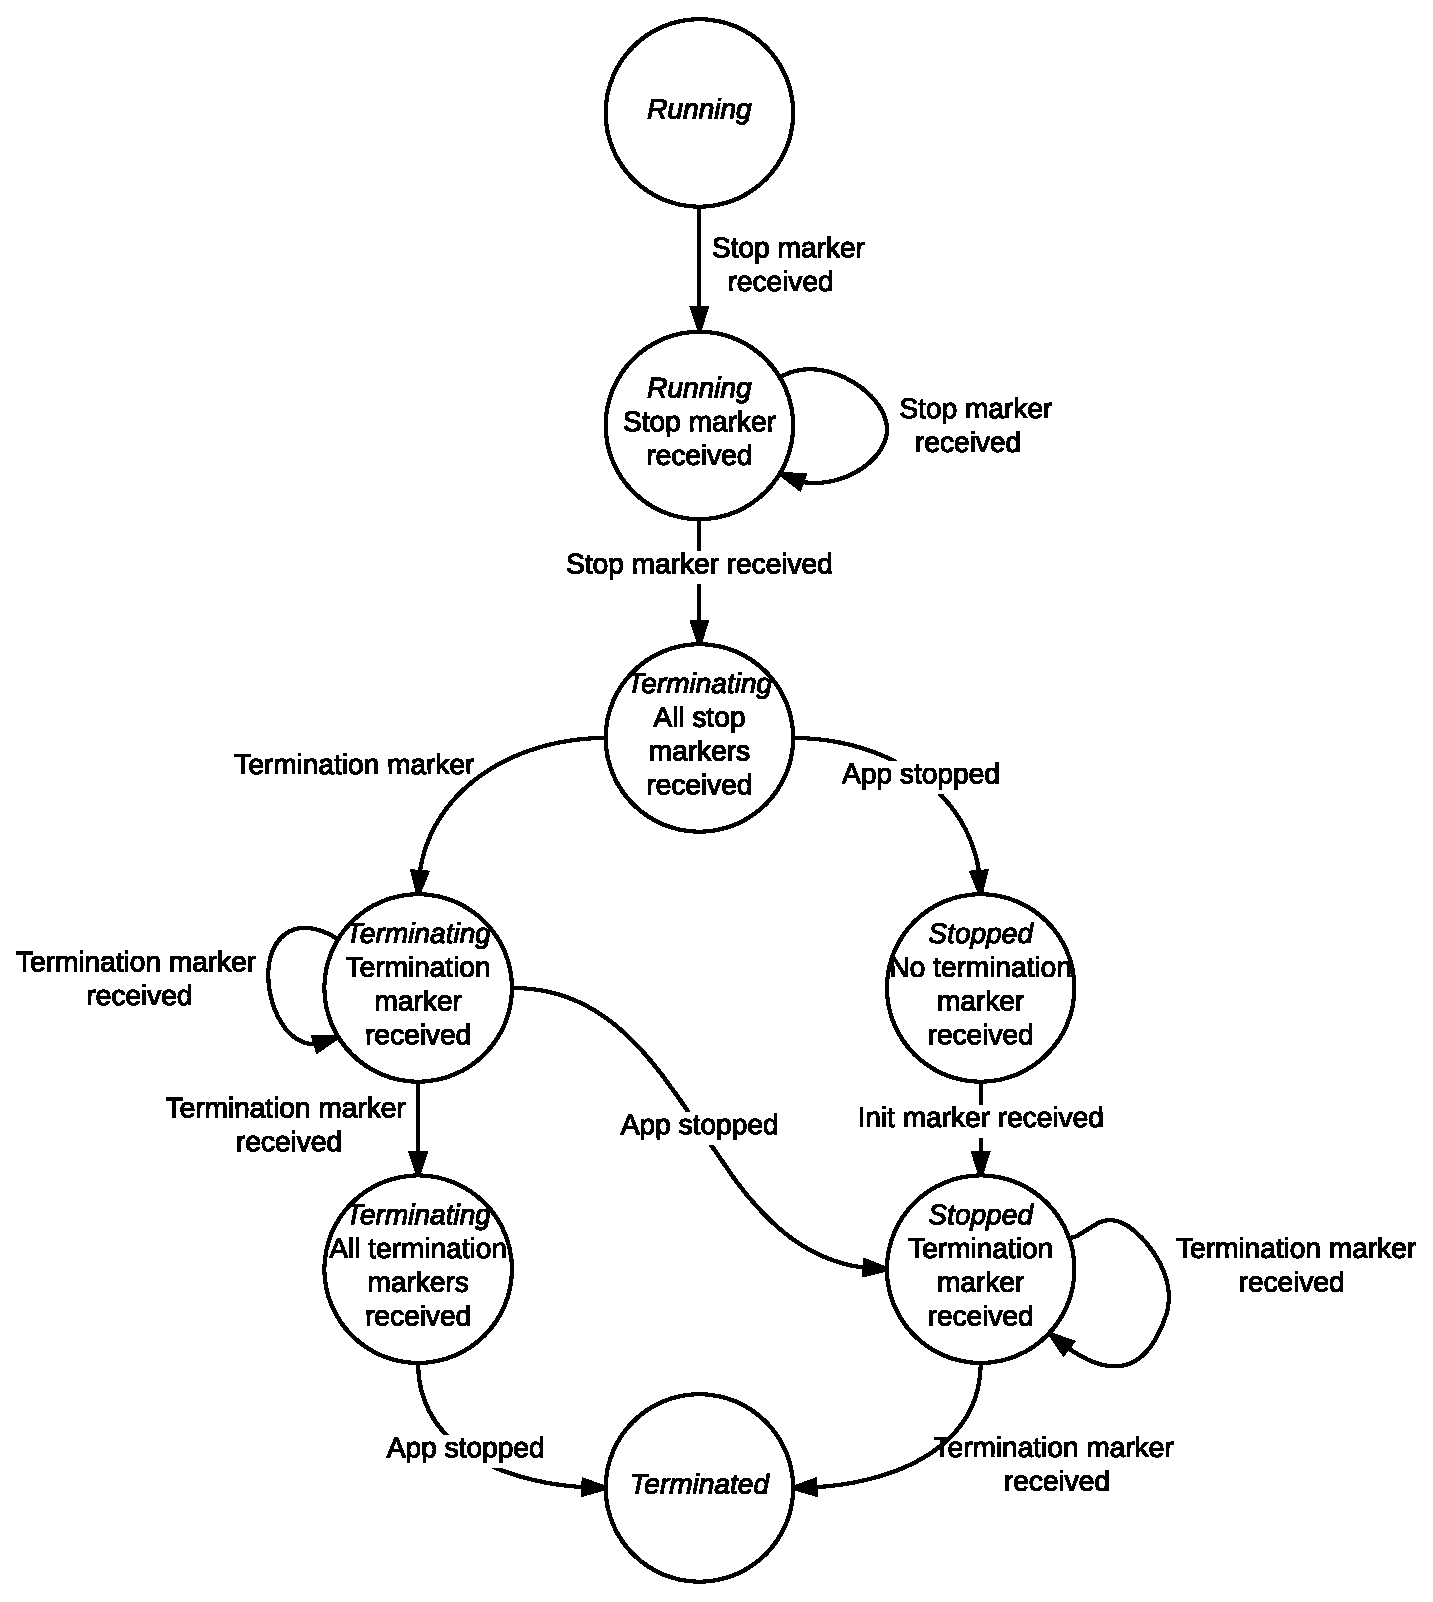
\includegraphics[width=.8\columnwidth]{images/solution/mw/termination.eps}
  \caption{Termination service: activity diagram}
  \label{fig:mw-termination}
\end{figure}
